
\documentclass[a4paper,10pt]{article}
\usepackage[top=2cm, left=2.5cm, right=2.5cm, bottom=2cm]{geometry}
\usepackage[cmex10]{amsmath}
\usepackage{graphicx}
\usepackage{gvv-book}
\usepackage{gvv}
\usepackage{textcomp}
\usepackage{multicol}

\begin{document}

\title{2013 - AR : Architecture and Planning Exam}
\author{Puni Aditya - EE25BTECH11046}
\date{11th August, 2025}
\maketitle
Duration: Three Hours \hfill Maximum Marks:100

\section*{Q.1 - Q.25 carry one mark each.}

\begin{enumerate}
    \item In case of residential apartments, the effective floor area available for use within an apartment, is known as 
    \begin{multicols}{2}
    \begin{enumerate}
        \item Carpet Area
        \item Built-up Area
        \item Plinth Area
        \item Super Built-up Area
    \end{enumerate}
    \end{multicols}
    \hfill (GATE-AR 2013)
    
    \item Star Rating of an Air Conditioner is determined by its 
    \begin{multicols}{2}
	\begin{enumerate}
        \item Power Consumption
        \item Energy Efficiency Ratio
        \item Cooling Capacity
        \item Power of Compressor
    \end{enumerate}
	\end{multicols}
    \hfill (GATE-AR 2013)
    
    \item V7 concept given by Le Corbusier refers to 
    \begin{multicols}{2}
	\begin{enumerate}
        \item Neighbourhood Planning
        \item Housing Typologies
        \item Architecture Design Principle
        \item Hierarchy of Roads
    \end{enumerate}
	\end{multicols}
    \hfill (GATE-AR 2013)
    
    \item In AUTOCAD, a line of infinite length in the direction defined by starting point and through point, is known as 
    \begin{multicols}{4}
	\begin{enumerate}
        \item RAY
        \item LINE
        \item PLINE
        \item XLINE
    \end{enumerate}
	\end{multicols}
    \hfill (GATE-AR 2013)
    
    \item Orbit Tower built at the London Olympic Park has been designed by 
    \begin{enumerate}
        \item Foster \& Partners
        \item Anish Kapoor \& Cecil Balmond
        \item Zaha Hadid \& Antony Gormley
        \item Richard Rogers \& Renzo Piano
    \end{enumerate}
    \hfill (GATE-AR 2013)
    
    \item As per National Building Code 2005, the minimum size of a habitable room in m$^2$ is 
    \begin{multicols}{4}
	\begin{enumerate}
        \item 9.5
        \item 10.5
        \item 11.5
        \item 12.5
    \end{enumerate}
	\end{multicols}
    \hfill (GATE-AR 2013)
    
    \item The urban form of Srirangam town in Tamil Nadu refers to 
    \begin{multicols}{4}
	\begin{enumerate}
        \item Dandaka
        \item Swastika
        \item Nandyavarta
        \item Sarvotabhadra
    \end{enumerate}
	\end{multicols}
    \hfill (GATE-AR 2013)
    
    \item PMGSY, a programme of Government of India, deals with 
    \begin{multicols}{2}
    \begin{enumerate}
        \item Urban Employment Generation
        \item Rural Employment Generation
        \item Rural Electrification
        \item Rural Road Development
    \end{enumerate}
    \end{multicols}
    \hfill (GATE-AR 2013)
    
    \item Beam or lowest division of the entablature which extends from column to column, is known as 
    \begin{multicols}{4}
	\begin{enumerate}
        \item Arabesque
        \item Arcade
        \item Architrave
        \item Arbour
    \end{enumerate}
	\end{multicols}
    \hfill (GATE-AR 2013)
    
    \item The information that is NOT essential to be submitted for sanction of any building plan is 
    \begin{multicols}{4}
	\begin{enumerate}
        \item Site Plan
        \item Floor Plans
        \item Title Deed
        \item Land Cost
    \end{enumerate}
	\end{multicols}
    \hfill (GATE-AR 2013)
    
    \item The tendency of an ecosystem to maintain its balance by regulatory mechanisms when disrupted, is known as 
    \begin{multicols}{4}
	\begin{enumerate}
        \item Homeostasis
        \item Entropy
        \item Succession
        \item Evolution
    \end{enumerate}
	\end{multicols}
    \hfill (GATE-AR 2013)
    
    \item Gantt Chart \textbf{DOES NOT} provide information about 
    \begin{multicols}{2}
	\begin{enumerate}
        \item List of Jobs
        \item Duration of Jobs
        \item Interdependency of Jobs
        \item Progress of Work
    \end{enumerate}
	\end{multicols}
    \hfill (GATE-AR 2013)

    \item If threshold of hearing has a sound level of zero decibels and the sound level in a broadcasting studio is 100 times the threshold of hearing, its value in decibels would be 
    \begin{multicols}{4}
	\begin{enumerate}
        \item 0
        \item 10
        \item 20
        \item 100
    \end{enumerate}
	\end{multicols}
    \hfill (GATE-AR 2013)

    \item The width to height ratio of the front facade of Parthenon (without the pediment) is 
    \begin{multicols}{2}
	\begin{enumerate}
        \item 9:4
        \item 4:9
        \item 1:1.618
        \item 1.618:1
    \end{enumerate}
	\end{multicols}
    \hfill (GATE-AR 2013)
    
    \item The face of an Icosahedron is 
    \begin{multicols}{2}
	\begin{enumerate}
        \item Equilateral Triangle
        \item Isosceles Triangle
        \item Square
        \item Pentagon
    \end{enumerate}
	\end{multicols}
    \hfill (GATE-AR 2013)

    \item The term 'Zeitgist', used in contemporary architecture, refers to 
    \begin{multicols}{4}
	\begin{enumerate}
        \item Iconicity
        \item Spirit of Times
        \item Kinesthetics
        \item Semantic Associations
    \end{enumerate}
	\end{multicols}
    \hfill (GATE-AR 2013)

    \item Alhambra, a UNESCO world heritage site, is classified as an example of 
    \begin{multicols}{2}
	\begin{enumerate}
        \item Moorish Architecture
        \item Mudejar Architecture
        \item Mozarabic Architecture
        \item Tudor Architecture
    \end{enumerate}
	\end{multicols}
    \hfill (GATE-AR 2013)

    \item Wythenshawe and Becontree are examples of 
    \begin{multicols}{2}
	\begin{enumerate}
        \item Factory Town
        \item Satellite Town
        \item Garden City
        \item Vertical Neighborhood
    \end{enumerate}
	\end{multicols}
    \hfill (GATE-AR 2013)

    \item National Ceremonial Plaza at Thimpu in Bhutan has been designed by 
    \begin{multicols}{2}
	\begin{enumerate}
        \item Christopher Charles Benninger
        \item Charles Correa
        \item Karan Grover
        \item I. M. Pei
    \end{enumerate}
	\end{multicols}
    \hfill (GATE-AR 2013)
    
    \item Physiochemical process of removing micro-organisms, colour and turbidity from sullage and sewage is known as 
    \begin{multicols}{2}
	\begin{enumerate}
        \item Putrefaction
        \item Clarification
        \item Liquefaction
        \item Infiltration
    \end{enumerate}
	\end{multicols}
    \hfill (GATE-AR 2013)

    \item Identify which is \textbf{NOT} a green building rating system 
    \begin{multicols}{4}
	\begin{enumerate}
        \item LEED
        \item CASBEE
        \item ENERGY BUILD
        \item BREEAM
    \end{enumerate}
	\end{multicols}
    \hfill (GATE-AR 2013)

    \item In 3DS Max, smooth 3D surfaces, by blending a series of selected shape curves, can be created by 
    \begin{multicols}{4}
	\begin{enumerate}
        \item Lofting
        \item Sweeping
        \item Filleting
        \item Extruding
    \end{enumerate}
	\end{multicols}
    \hfill (GATE-AR 2013)

    \item Travel behavior characteristics of an urban area can be derived from 
    \begin{multicols}{2}
	\begin{enumerate}
        \item Parking Survey
        \item Demographic Survey
        \item Socio Economic Survey
        \item Origin \& Destination Survey
    \end{enumerate}
	\end{multicols}
    \hfill (GATE-AR 2013)

    \item In GIS, the set of entities representing vector data type is 
    \begin{enumerate}
        \item Point, Line, Polygon, TIN
        \item Pixel, Voxel
        \item DEM, DSM, DTM
        \item Coordinates, Elevation, Slope
    \end{enumerate}
    \hfill (GATE-AR 2013)

    \item A common flowering shrub is 
    \begin{multicols}{4}
	\begin{enumerate}
        \item Tectona grandis
        \item Mimusops elengi
        \item Dalbergia sisso
        \item Ixora coccinea
    \end{enumerate}
	\end{multicols}
    \hfill (GATE-AR 2013)

\section*{Q.26 to Q.55 carry two marks each.}

    \item The correct arrangement of the height of towers given below in \textbf{descending order} is
    \begin{itemize}
    \item Burj Khalifa, Dubai
    \item Petronas Tower, Kuala Lumpur
    \item Taipei 101, Taiwan
    \item Bank of China Tower, Hong Kong
    \end{itemize}
    \begin{multicols}{2}
	\begin{enumerate}
        \item P, Q, R, S
        \item P, Q, S, R
        \item P, R, S, Q
        \item P, R, Q, S
    \end{enumerate}
	\end{multicols}
    \hfill (GATE-AR 2013)

    \item Match the buildings in \textbf{Group I} with their corresponding architects in \textbf{Group II} \\
    \begin{tabular}{ l l }
	\textbf{Group I} & \textbf{Group II} \\
	P. Khalsa Heritage Complex, Anandpur Sahib & 1. Philip Johnson \\
	Q. Lisbon Ismaili Centre, Lisbon & 2. Charles Correa \\
	R. Neuroscience Centre, Cambridge, USA & 3. Raj Rewal \\
	S. National Centre for Performing Arts, Mumbai & 4. B. V. Doshi \\
	& 5. Moshe Safdie \\
	\end{tabular}
	\begin{multicols}{2}
	\begin{enumerate}
        \item P-2, Q-5, R-1, S-4
        \item P-5, Q-3, R-2, S-1
        \item P-4, Q-2, R-1, S-3
        \item P-5, Q-2, R-1, S-4
    \end{enumerate}
	\end{multicols}
    \hfill (GATE-AR 2013)

    \item The term 'Working head' in context of water supply system means 
    \begin{enumerate}
        \item Height of a body of water falling freely under the force of gravity to acquire a certain velocity
        \item Rate of increase of velocity with respect to distance normal to the direction of flow
        \item Total head with deduction for velocity head or losses
        \item Difference between supply and delivery water levels
    \end{enumerate}
    \hfill (GATE-AR 2013)

    \item In a theoretical traffic flow relationship, as shown in the figure given below, the slope of line \textbf{OF} joining point F on the curve and the origin \textbf{O} represents \\
    \begin{figure}[h!]
    \centering
    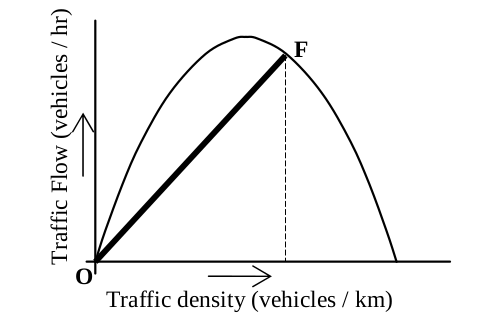
\includegraphics[width=0.5\linewidth]{figs/01.jpg}
    \caption{Theoretical Traffic Flow Relationship}
    \label{fig:Img01}
    \end{figure}
    \begin{multicols}{2}
	\begin{enumerate}
        \item Corresponding space mean speed
        \item Speed at maximum flow
        \item Travel time at corresponding density
        \item Average headway at corresponding flow
    \end{enumerate}
	\end{multicols}
    \hfill (GATE-AR 2013)

    \item Match the CAD terms in \textbf{Group I} with their corresponding functions in \textbf{Group II} \\
    \begin{tabular}{ l l }
	\textbf{Group I} & \textbf{Group II} \\
	P. Tiled viewport & 1. Boolean operator \\
	Q. UCS & 2. Solid model \\
	R. DXF & 3. Coordinate system \\
	S. Extrude & 4. Drawing interchange format \\
	& 5. Model space \\
	\end{tabular}
	\begin{multicols}{2}
	\begin{enumerate}
        \item P-4, Q-3, R-2, S-1
        \item P-2, Q-5, R-2, S-1
        \item P-5, Q-3, R-4, S-2
        \item P-3, Q-5, R-4, S-2
    \end{enumerate}
	\end{multicols}
    \hfill (GATE-AR 2013)

    \item Match the historic periods in \textbf{Group I} with their corresponding examples of towns in \textbf{Group II} \\
    \begin{tabular}{ l l }
	\textbf{Group I} & \textbf{Group II} \\
	P. Egyptian & 1. Miletus \\
	Q. Greek & 2. Montpazier \\
	R. Medieval & 3. Kahun \\
	S. Renaissance & 4. Versailles \\
	& 5. Timgad \\
	\end{tabular}
	\begin{multicols}{2}
	\begin{enumerate}
        \item P-3, Q-1, R-2, S-4
        \item P-3, Q-1, R-4, S-5
        \item P-4, Q-1, R-5, S-2
        \item P-5, Q-1, R-3, S-2
    \end{enumerate}
	\end{multicols}
    \hfill (GATE-AR 2013)

    \item Match the components of an Indian urban land use map in \textbf{Group I} with their corresponding colour codes as per UDPFI guidelines in \textbf{Group II} \\
    \begin{tabular}{ l l }
	\textbf{Group I} & \textbf{Group II} \\
	P. Public / Semipublic & 1. Violet \\
	Q. Industry & 2. Grey \\
	R. Transportation & 3. Red \\
	S. Commercial & 4. Blue \\
	& 5. Yellow \\
	\end{tabular}
	\begin{multicols}{2}
	\begin{enumerate}
        \item P-1, Q-3, R-2, S-5
        \item P-2, Q-1, R-3, S-4
        \item P-3, Q-4, R-5, S-2
        \item P-3, Q-1, R-2, S-4
    \end{enumerate}
	\end{multicols}
    \hfill (GATE-AR 2013)

    \item Match the books in \textbf{Group I} with their corresponding authors in \textbf{Group II} \\
    \begin{tabular}{ l l }
	\textbf{Group I} & \textbf{Group II} \\
	P. Design of Cities & 1. Amos Rapoport \\
	Q. On the Cultural Origin of Settlements & 2. Leo Jacobson and Ved Prakash \\
	R. Urbanization and National Development & 3. Edmond Bacon \\
	S. Planning Theory & 4. Christopher Alexander \\
	& 5. Andreas Faludi \\
	\end{tabular}
	\begin{multicols}{2}
	\begin{enumerate}
        \item P-3, Q-4, R-1, S-5
        \item P-3, Q-1, R-2, S-5
        \item P-4, Q-3, R-5, S-2
        \item P-3, Q-4, R-1, S-2
    \end{enumerate}
	\end{multicols}
    \hfill (GATE-AR 2013)

    \item Match the temples in \textbf{Group I} with their corresponding historical periods in \textbf{Group II} \\
    \begin{tabular}{ l l }
	\textbf{Group I} & \textbf{Group II} \\
	P. Vaikuntha Perumal Temple, Kancheepuram & 1. Vijaynagara \\
	Q. Meenakshi Temple, Madurai & 2. Chalukya \\
	R. Durga Temple, Aihole & 3. Chola \\
	S. Brihadeshwara Temple, Thanjavur & 4. Pandya \\
	& 5. Pallava \\
	\end{tabular}
	\begin{multicols}{2}
	\begin{enumerate}
        \item P-2, Q-3, R-5, S-1
        \item P-5, Q-1, R-4, S-3
        \item P-3, Q-5, R-2, S-1
        \item P-5, Q-4, R-2, S-3
    \end{enumerate}
	\end{multicols}
    \hfill (GATE-AR 2013)

    \item Match the theories in \textbf{Group I} with their corresponding propagators in \textbf{Group II} \\
    \begin{tabular}{ l l }
	\textbf{Group I} & \textbf{Group II} \\
	P. Choice theory of planning & 1. Paul Davidoff and T.A. Reiner \\
	Q. Connurbation & 2. Patrick Geddes \\
	R. Classical theory of land use & 3. Homer Hoyt \\
	S. Central place theory & 4. Richard L. Meier \\
	& 5. Walter Christaller \\
	\end{tabular}
	\begin{multicols}{2}
	\begin{enumerate}
        \item P-2, Q-3, R-5, S-1
        \item P-1, Q-2, R-4, S-5
        \item P-4, Q-3, R-5, S-2
        \item P-5, Q-4, R-3, S-2
    \end{enumerate}
	\end{multicols}
    \hfill (GATE-AR 2013)

    \item Match the buildings in \textbf{Group I} with their corresponding structural feature in \textbf{Group II} \\
    \begin{tabular}{ l l }
	\textbf{Group I} & \textbf{Group II} \\
	P. Yokohama Port Terminal, Yokohama & 1. Geodesic Dome \\
	Q. Stanstead Airport, London & 2. Shell Structure \\
	R. TWA Terminal, New York & 3. Space Frame \\
	S. Montreal Biosphere, Montreal & 4. Folded Steel Plate Structure \\
	& 5. Pneumatic Structure \\
	\end{tabular}
	\begin{multicols}{2}
	\begin{enumerate}
        \item P-4, Q-3, R-2, S-1
        \item P-2, Q-1, R-3, S-4
        \item P-4, Q-3, R-5, S-2
        \item P-5, Q-3, R-4, S-2
    \end{enumerate}
	\end{multicols}
    \hfill (GATE-AR 2013)

    \item Match the Five Year Plans listed under \textbf{Group I} with their corresponding feature from \textbf{Group II} \\
    \begin{tabular}{ l l }
	\textbf{Group I} & \textbf{Group II} \\
	P. First Five Year Plan & 1. Formation of HUDCO \\
	Q. Fourth Five Year Plan & 2. Establishment of TCPO \\
	R. Seventh Five Year Plan & 3. Introduction of JNNURM \\
	S. Tenth Five Year Plan & 4. Announcement of National Housing Policy \\
	& 5. Passing of Urban Land Ceiling and Regulation Act \\
	\end{tabular}
	\begin{multicols}{2}
	\begin{enumerate}
        \item P-5,Q-2,R-4,S-3
        \item P-2,Q-1,R-4,S-3
        \item P-4,Q-1,R-2,S-5
        \item P-1,Q-2,R-3,S-5
    \end{enumerate}
	\end{multicols}
    \hfill (GATE-AR 2013)

    \item Match the landscape designers listed under \textbf{Group I} with their appropriate contribution from \textbf{Group II} \\
    \begin{tabular}{ l l }
	\textbf{Group I} & \textbf{Group II} \\
	P. Lancelot 'Capability' Brown & 1. The Well-tempered Garden \\
	Q. Andre Le Notre & 2. Kew Garden \\
	R. Joseph Paxton & 3. Versailles Garden \\
	S. Frederick Law Olmstead & 4. Crystal Palace \\
	& 5. Central Park \\
	\end{tabular}
	\begin{multicols}{2}
	\begin{enumerate}
        \item P-3, Q-1, R-4, S-2
        \item P-5, Q-3, R-4, S-2
        \item P-3, Q-1, R-2, S-5
        \item P-2, Q-3, R-4, S-5
    \end{enumerate}
	\end{multicols}
    \hfill (GATE-AR 2013)

    \item Match the organism type from \textbf{Group I} with the appropriate example from \textbf{Group II} \\
    \begin{tabular}{ l l }
	\textbf{Group I} & \textbf{Group II} \\
	P. Autotroph & 1. Nitrifying Bacteria \\
	Q. Heterotroph & 2. Grasshopper \\
	R. Chemotroph & 3. Grass \\
	S. Saprophyte & 4. Vulture \\
	& 5. Fungus \\
	\end{tabular}
	\begin{multicols}{2}
	\begin{enumerate}
        \item P-5, Q-4, R-1, S-2
        \item P-2, Q-1, R-5, S-4
        \item P-1, Q-2, R-4, S-5
        \item P-3, Q-2, R-1, S-5
    \end{enumerate}
	\end{multicols}
    \hfill (GATE-AR 2013)

    \item Match the concepts in \textbf{Group I} with their corresponding authors in \textbf{Group II} \\
    \begin{tabular}{ l l }
	\textbf{Group I} & \textbf{Group II} \\
	P. Proxemics Theory & 1. Gordon Cullen \\
	Q. Serial Vision & 2. Edward T. Hall \\
	R. Urban Imageability & 3. Oscar Newman \\
	S. Defensible Space & 4. Paul Zucker \\
	& 5. Kevin Lynch \\
	\end{tabular}
	\begin{multicols}{2}
	\begin{enumerate}
        \item P-2, Q-1, R-5, S-3
        \item P-2, Q-1, R-3, S-4
        \item P-4, Q-1, R-5, S-2
        \item P-3, Q-5, R-2, S-1
    \end{enumerate}
	\end{multicols}
    \hfill (GATE-AR 2013)

    \item If the area coverage of one sprinkler is 20 m$^2$, with a maximum and minimum spacing of 4.6 m and 1.8 m respectively, the minimum number of sprinklers required to be arranged in a regular orthogonal grid to cover the area of a 15 m $\times$ 20 m room would be \rule{3cm}{0.4pt}.
    \hfill (GATE-AR 2013)

    \item If the slope of a hipped roof is 60 degrees and height of the roof is 3 m, span of the room, in m, would be \rule{3cm}{0.4pt}.
    \hfill (GATE-AR 2013)

    \item Volume of coarse aggregate in m$^3$ present in 1.0 m$^3$ of 1 : 1.5 : 3 concrete mix made by volume batching is \rule{3cm}{0.4pt}.
    \hfill (GATE-AR 2013)

    \item A tank of internal dimension 3 m $\times$ 5 m $\times$ 4 m (Length $\times$ Breadth $\times$ Height) has 200 mm thick brick wall on all sides. Volume of brickwork in m$^3$ would be \rule{3cm}{0.4pt}.
    \hfill (GATE-AR 2013)

    \item Flux emitted from a 1cd light source in all directions, in lumens, would be \rule{3cm}{0.4pt}.
    \hfill (GATE-AR 2013)

    \item 50 Hectare of residential sector has 65\% buildable area. The FAR of the buildable area is 1.5. Within the residential sector, 60\% of dwelling units are of area 100 m$^2$ each and 40\% of the dwelling units are of area 80 m$^2$ each. \\
    The gross residential density, in dwelling units per Hectare, would be \rule{3cm}{0.4pt}.
    \hfill (GATE-AR 2013)

    \item In the given project network diagram, the total slack for job A in days would be \rule{3cm}{0.4pt}.
    \begin{figure}[h!]
    \centering
    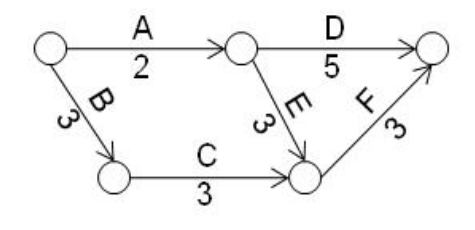
\includegraphics[width=0.5\linewidth]{figs/02.jpg}
    \caption{Project Network Diagram}
    \label{fig:Img02}
    \end{figure}
    \hfill (GATE-AR 2013)

\section*{Common Data Questions}
\section*{Common Data for Questions 48 and 49:}
\subsection*{The scale of a contour map is 1:10,000 and the contour interval is 5 m. Distance between two given points on the map is 2 cm and the elevation difference between the two given points is 10 m.}

    \item The actual distance between the two given points in m would be
    \begin{multicols}{4}
	\begin{enumerate}
        \item 2
        \item 20
        \item 200
        \item 2000
    \end{enumerate}
	\end{multicols}
    \hfill (GATE-AR 2013)

    \item The slope between two given points in percentage is
    \begin{multicols}{4}
	\begin{enumerate}
        \item 5
        \item 10
        \item 15
        \item 20
    \end{enumerate}
	\end{multicols}
    \hfill (GATE-AR 2013)

\section*{Common Data for Questions 50 and 51:}
\subsection*{A point load of 3kN acts at mid-span of a 4 m long cantilever beam as shown in figure below.}
	\begin{figure}[h!]
    \centering
    
\includegraphics[width=0.5\linewidth]{figs/03.jpg}
    \caption{Cantilever Beam}
    \label{fig:Img03}
    \end{figure}
    
    \item Shearing force at free end in kN is
    \begin{multicols}{4}
	\begin{enumerate}
        \item 0
        \item 3
        \item 6
        \item 12
    \end{enumerate}
	\end{multicols}
    \hfill (GATE-AR 2013)

    \item Bending moment at mid-span in kNm is
    \begin{multicols}{4}
	\begin{enumerate}
        \item 0
        \item 2
        \item 4
        \item 6
    \end{enumerate}
	\end{multicols}
    \hfill (GATE-AR 2013)

\section*{Linked Answer Questions}

\section*{Statement for Linked Answer Questions 52 and 53:}
\subsection*{Cost of a new building is Rs 10,00,000 and its scrap value after 50 years is Rs. 1,00,000. Using straight line method}

    \item The annual depreciation of the building in Rs. would be
    \begin{multicols}{4}
	\begin{enumerate}
        \item 10,000
        \item 15,000
        \item 18,000
        \item 20,000
    \end{enumerate}
	\end{multicols}
    \hfill (GATE-AR 2013)

    \item The book value after 10 years in Rs. would be
    \begin{multicols}{4}
	\begin{enumerate}
        \item 1,80,000
        \item 3,60,000
        \item 6,00,000
        \item 8,20,000
    \end{enumerate}
	\end{multicols}
    \hfill (GATE-AR 2013)

\section*{Statement for Linked Answer Questions 54 and 55:}
\subsection*{A room of size 100 m$^2$ is illuminated by 10 lamps of 40 W having a luminous efficacy of 50 lm/W.}

    \item Total flux emitted by the lamps in lumens would be
    \begin{multicols}{4}
	\begin{enumerate}
        \item 2,000
        \item 5,000
        \item 10,000
        \item 20,000
    \end{enumerate}
	\end{multicols}
    \hfill (GATE-AR 2013)

    \item If utilization factor is 0.5, at a working height of 90 cm above the floor level, the illumination in lux would be
    \begin{multicols}{4}
	\begin{enumerate}
        \item 100
        \item 200
        \item 500
        \item 1000
    \end{enumerate}
	\end{multicols}
    \hfill (GATE-AR 2013)

\section*{General Aptitude (GA) Questions}

\section*{Q.56 - Q.60 carry one mark each.}

    \item A number is as much greater than 75 as it is smaller than 117. The number is:
    \begin{multicols}{4}
	\begin{enumerate}
        \item 91
        \item 93
        \item 89
        \item 96
    \end{enumerate}
	\end{multicols}
    \hfill (GATE-AR 2013)

    \item \begin{tabular}{ l l l l }
    The professor & ordered to & the students to go & out of the class. \\
    I & II & III & IV \\
    \end{tabular}
    Which of the above underlined parts of the sentence is grammatically incorrect?
    \begin{multicols}{4}
	\begin{enumerate}
        \item I
        \item II
        \item III
        \item IV
    \end{enumerate}
	\end{multicols}
    \hfill (GATE-AR 2013)

    \item Which of the following options is the closest in meaning to the word given below: \\
    Primeval
    \begin{multicols}{4}
	\begin{enumerate}
        \item Modern
        \item Historic
        \item Primitive
        \item Antique
    \end{enumerate}
	\end{multicols}
    \hfill (GATE-AR 2013)

    \item Friendship, no matter how \rule{2cm}{0.4pt} it is, has its limitations.
    \begin{enumerate}
        \item cordial
        \item intimate
        \item secret
        \item pleasant
    \end{enumerate}
    \hfill (GATE-AR 2013)

    \item Select the pair that best expresses a relationship similar to that expressed in the pair: \\
    \textbf{Medicine: Health}
    \begin{multicols}{2}
	\begin{enumerate}
        \item Science: Experiment
        \item Wealth: Peace
        \item Education: Knowledge
        \item Money: Happiness
    \end{enumerate}
	\end{multicols}
    \hfill (GATE-AR 2013)

\section*{Q.61 to Q.65 carry two marks each.}

    \item X and Y are two positive real numbers such that $2X + Y \leq 6$ and $X + 2Y \leq 8$. For which of the following values of $(X,Y)$ the function $f(X,Y) = 3X + 6Y$ will give maximum value?
    \begin{enumerate}
        \item (4/3, 10/3)
        \item (8/3, 20/3)
        \item (8/3, 10/3)
        \item (4/3, 20/3)
    \end{enumerate}
    \hfill (GATE-AR 2013)

    \item If $|4X - 7| = 5$ then the values of $2|X| - |-X|$ is:
    \begin{multicols}{4}
	\begin{enumerate}
        \item 2, 1/3
        \item 1/2, 3
        \item 3/2, 9
        \item 2/3, 9
    \end{enumerate}
	\end{multicols}
    \hfill (GATE-AR 2013)

    \item Following table provides figures (in rupees) on annual expenditure of a firm for two years - 2010 and 2011. \\
    \begin{center}
	\begin{tabular}{ | l | c | c | }
	\hline
	\textbf{Category} & \textbf{2010} & \textbf{2011} \\
	\hline
	Raw material & 5200 & 6240 \\
	\hline
	Power \& fuel & 7000 & 9450 \\
	\hline
	Salary \& wages & 9000 & 12600 \\
	\hline
	Plant \& machinery & 20000 & 25000 \\
	\hline
	Advertising & 15000 & 19500 \\
	\hline
	Research \& Development & 22000 & 26400 \\
	\hline
	\end{tabular}
	\end{center}
    In 2011, which of the following two categories have registered increase by same percentage?
    \begin{enumerate}
        \item Raw material and Salary \& wages
        \item Salary \& wages and Advertising
        \item Power \& fuel and Advertising
        \item Raw material and Research \& Development
    \end{enumerate}
    \hfill (GATE-AR 2013)

    \item A firm is selling its product at Rs. 60 per unit. The total cost of production is Rs. 100 and firm is earning total profit of Rs. 500. Later, the total cost increased by 30\%. By what percentage the price should be increased to maintained the same profit level.
    \begin{multicols}{4}
	\begin{enumerate}
        \item 5
        \item 10
        \item 15
        \item 30
    \end{enumerate}
	\end{multicols}
    \hfill (GATE-AR 2013)

    \item Abhishek is elder to Savar. \\
    Savar is younger to Anshul. \\
    Which of the given conclusions is logically valid and is inferred from the above statements?
    \begin{enumerate}
        \item Abhishek is elder to Anshul
        \item Anshul is elder to Abhishek
        \item Abhishek and Anshul are of the same age
        \item No conclusion follows
    \end{enumerate}
    \hfill (GATE-AR 2013)

\end{enumerate}

\centering
\section*{END OF THE QUESTION PAPER}

\end{document}
